\documentclass[a4paper,12pt]{article}
\usepackage[utf8]{inputenc}
\usepackage{geometry}
\usepackage{fancyhdr}
\usepackage{listings}
\usepackage{xcolor}
\usepackage{graphicx}
\usepackage{float}
\usepackage{amsmath}

% Margins
\geometry{left=15mm, right=15mm, top=25mm, bottom=15mm}

% Header/Footer
\pagestyle{fancy}
\fancyhf{}
\renewcommand{\headrulewidth}{0pt}
\rfoot{Page \thepage}

\fancypagestyle{firstpage}{
    \fancyhf{}
    \lhead{
        \small \textbf{Name:} Mrigaj Shaw \\ 
        \small \textbf{Roll No:} 2024CSB041
    }
    \chead{\LARGE \textbf{Assignment 7}} 
    \rfoot{Page \thepage}
    \renewcommand{\headrulewidth}{1pt}
}

% Code Style
\definecolor{codegreen}{rgb}{0,0.6,0}
\definecolor{codegray}{rgb}{0.5,0.5,0.5}
\definecolor{codepurple}{rgb}{0.58,0,0.82}
\definecolor{backcolour}{rgb}{0.95,0.95,0.92}

\lstdefinestyle{MyCodeStyle}{
    backgroundcolor=\color{backcolour},   
    commentstyle=\color{codegreen},
    keywordstyle=\color{magenta},
    numberstyle=\tiny\color{codegray},
    stringstyle=\color{codepurple},
    basicstyle=\ttfamily\footnotesize,
    breakatwhitespace=false,         
    breaklines=true,                 
    keepspaces=true,                 
    numbers=left,                    
    numbersep=5pt,                  
    showspaces=false,                
    showstringspaces=false,
    showtabs=false,                  
    tabsize=4
}
\lstset{style=MyCodeStyle}

\begin{document}
\thispagestyle{firstpage}

% --- Problem 1 ---
\section*{Problem 1}
\textbf{Problem Statement:} In this assignment, you will design and implement a smart navigation system for a city with 10 locations (vertices) such as schools, hospitals, and markets. The roads between these locations are represented as edges:
$$E=\{(u,v,w)|w_{i}>0\}$$
where each edge has a positive travel cost (distance or time). Dynamically construct the directed graph and compute the shortest path from a selected source location using two different approaches: adjacency list representation and adjacency matrix representation.

\textbf{Your task:}
\begin{enumerate}
    \item \textbf{Graph Construction}
    \begin{itemize}
        \item Define the vertex set: $V=\{v_{1},v_{2},...,v_{10}\}$
        \item Dynamically construct the graph by allowing the user to:
        \begin{itemize}
            \item Select any two vertices $(u, v)$
            \item Assign a positive weight $w_{i}>0$
        \end{itemize}
        \item Represent the same graph in two formats:
        \begin{itemize}
            \item Adjacency List Representation
            \item Adjacency Matrix Representation
        \end{itemize}
    \end{itemize}
    \item \textbf{Scenario 1: Adjacency List + Min-Heap}
    \begin{itemize}
        \item Implement Dijkstra's Algorithm using adjacency list
        \item Use a min-heap (priority queue) to select the next vertex with minimum distance
        \item Compute the shortest path from a chosen source vertex to all other vertices
    \end{itemize}
    \item \textbf{Scenario 2: Adjacency Matrix + Min-Heap}
    \begin{itemize}
        \item Implement Dijkstra's Algorithm using adjacency matrix
        \item Use a min-heap for selecting the next vertex
        \item Compute the shortest path from the same source vertex
    \end{itemize}
    \item \textbf{Performance Evaluation}
    \begin{itemize}
        \item Execute both implementations on the same graph input and measure:
        \begin{itemize}
            \item Execution time $t$
        \end{itemize}
        \item Perform analysis under:
        \begin{itemize}
            \item Sparse Graph (few edges)
            \item Dense Graph (many edges)
        \end{itemize}
    \end{itemize}
\end{enumerate}

\newpage
\subsection*{Code}
\lstinputlisting[language=C]{Problem1/SmartNavigationCity.c}

\newpage
\subsection*{Output}
\begin{figure}[H]
    \centering
    
\includegraphics[width=0.9\textwidth]{Problem1/Problem1.png}
\end{figure}
\begin{figure}[H]
    \centering
    
\includegraphics[width=0.9\textwidth]{Problem1/Problem1_1.png}
\end{figure}
\begin{figure}[H]
    \centering
    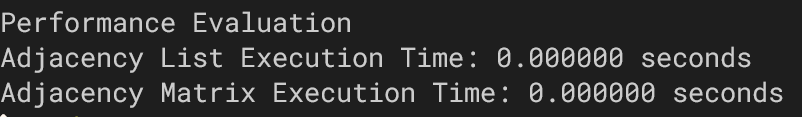
\includegraphics[width=0.9\textwidth]{Problem1/Problem1_1_Sparse.png}
\end{figure}
\begin{figure}[H]
    \centering
    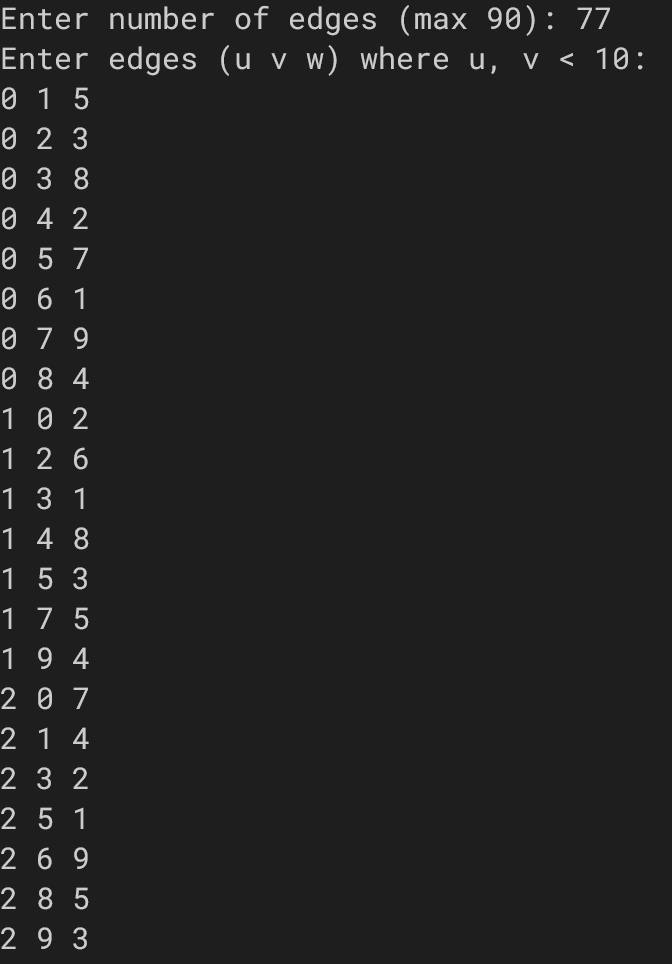
\includegraphics[width=0.9\textwidth]{Problem1/Problem1_2_1.png}
\end{figure}
\begin{figure}[H]
    \centering
    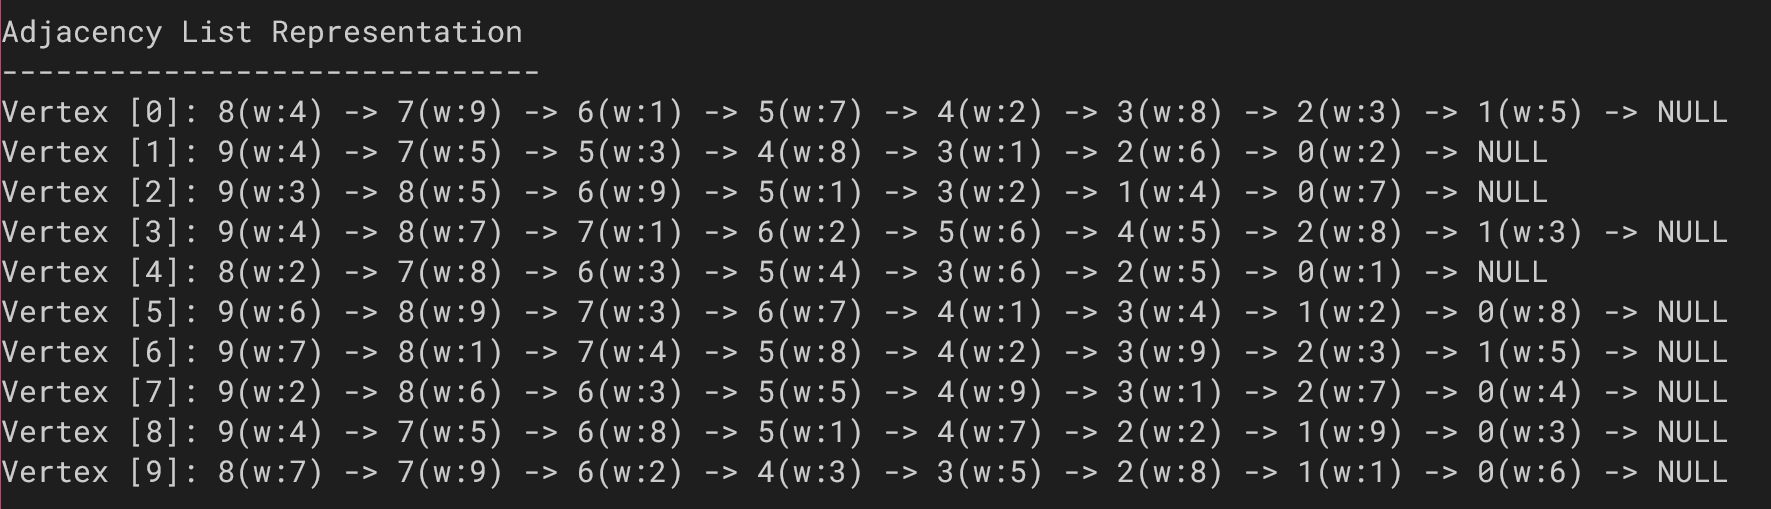
\includegraphics[width=0.9\textwidth]{Problem1/Problem1_2_2_ListRepresentation.png}
\end{figure}
\begin{figure}[H]
    \centering
    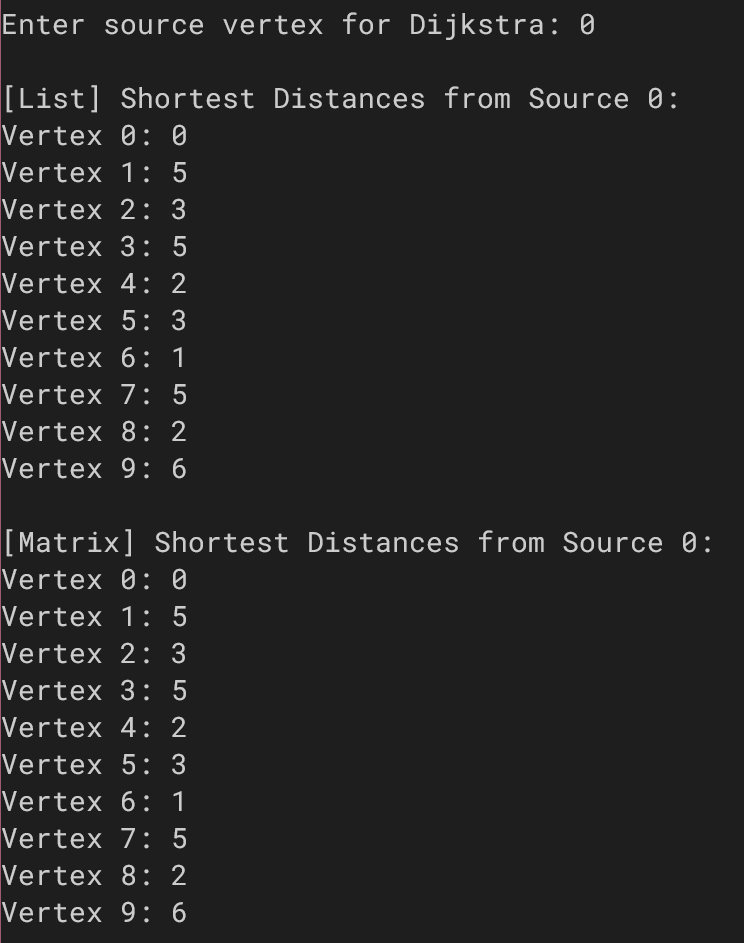
\includegraphics[width=0.9\textwidth]{Problem1/Problem1_2_3.png}
\end{figure}
\begin{figure}[H]
    \centering
    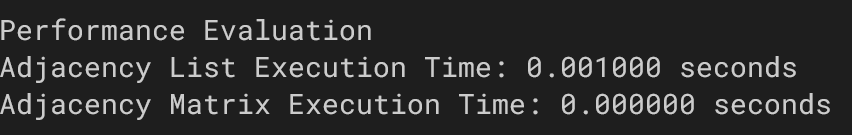
\includegraphics[width=0.9\textwidth]{Problem1/Problem1_2_4.png}
\end{figure}

\newpage
\subsection*{Inference}
\begin{itemize}
    \item \textbf{Time Complexity (Adjacency List):} $O((V + E) \log V)$. This approach is highly efficient for extracting the minimum distance node and iterating only through the existing neighbors.
    \item \textbf{Time Complexity (Adjacency Matrix):} $O(V^2 + E \log V)$. Even with a min-heap, the matrix requires iterating over all $V$ possible vertices to find connected neighbors, making it strictly bounded by $O(V^2)$.
    \item \textbf{Sparse vs. Dense Graph Performance:} For sparse graphs ($E \approx V$), the adjacency list implementation executes significantly faster and consumes less memory. For dense graphs ($E \approx V^2$), the adjacency matrix implementation performs competitively, though the list representation remains mathematically optimal.
\end{itemize}

\newpage

% --- Problem 2 ---
\section*{Problem 2}
\textbf{Problem Statement:} In this assignment, you will explore an important limitation of Dijkstra's Algorithm by designing a graph with $V=10$ vertices where the user dynamically constructs edges $E=\{(u,v,w)\}$, including the possibility of negative edge weights and even a negative weight cycle. While Dijkstra's Algorithm assumes $w_{i}>0$, you will intentionally violate this condition by allowing $w_{i}<0$ and analyze how the algorithm fails to compute correct shortest paths from a source vertex $s$.

Dijkstra relies on the greedy assumption that once a node $u$ is selected with minimum distance, its shortest path is finalized. However, in the presence of negative edges, this assumption breaks:
$$\exists(u,v)\in E \text{ such that } w(u,v)<0 \Rightarrow dist[v]<dist[u]+w(u,v)$$
even after node $u$ has already been processed.

\textbf{Negative Cycle Condition} \\
If a negative cycle exists such that $\sum_{(u,v)\in C}w(u,v)<0$, then the shortest path becomes undefined because distances can decrease indefinitely: $dist[v]\rightarrow-\infty$.

\textbf{Your task:}
\begin{itemize}
    \item Dynamically create a graph with 10 vertices
    \item Add edges between vertices, including negative weights
    \item Intentionally create a cycle with total negative weight
    \item Apply Dijkstra's Algorithm from a source vertex
    \item Observe incorrect results or failure to detect the negative cycle
\end{itemize}

\newpage
\subsection*{Code}
\lstinputlisting[language=C]{Problem2/DijkstraLimitationNegativeEdgeWeightCycle.c}

\newpage
\subsection*{Output}
\begin{figure}[H]
    \centering
    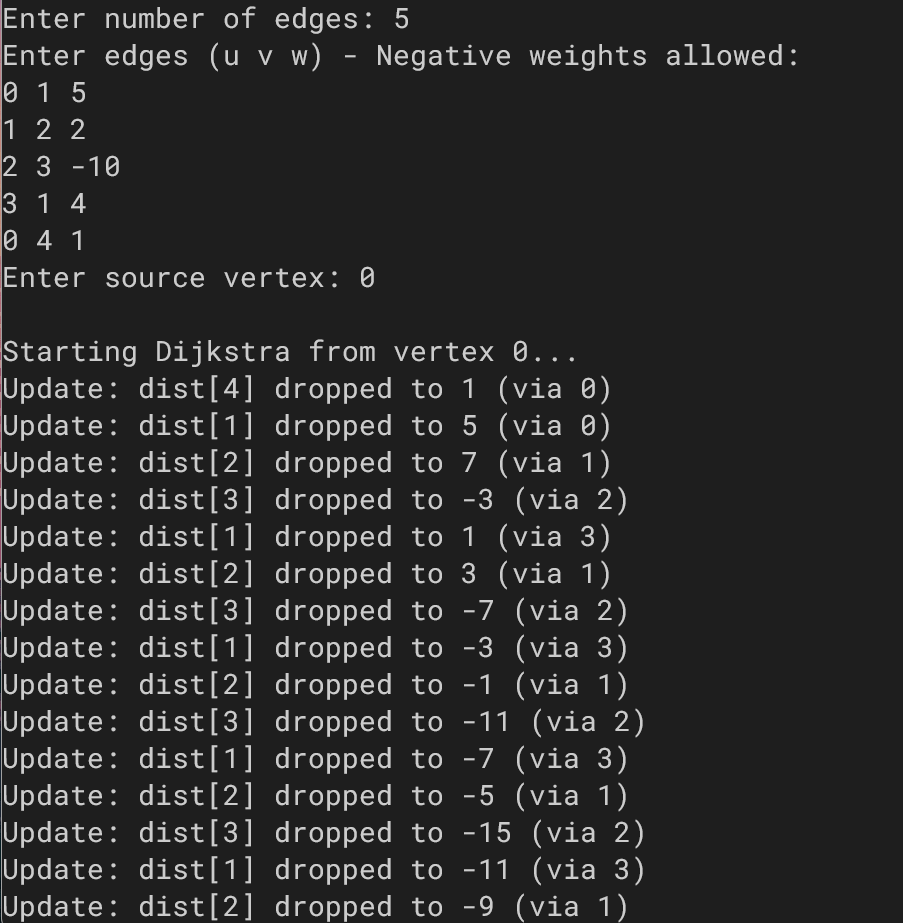
\includegraphics[width=0.9\textwidth]{Problem2/Problem2_1.png}
\end{figure}
\begin{figure}[H]
    \centering
    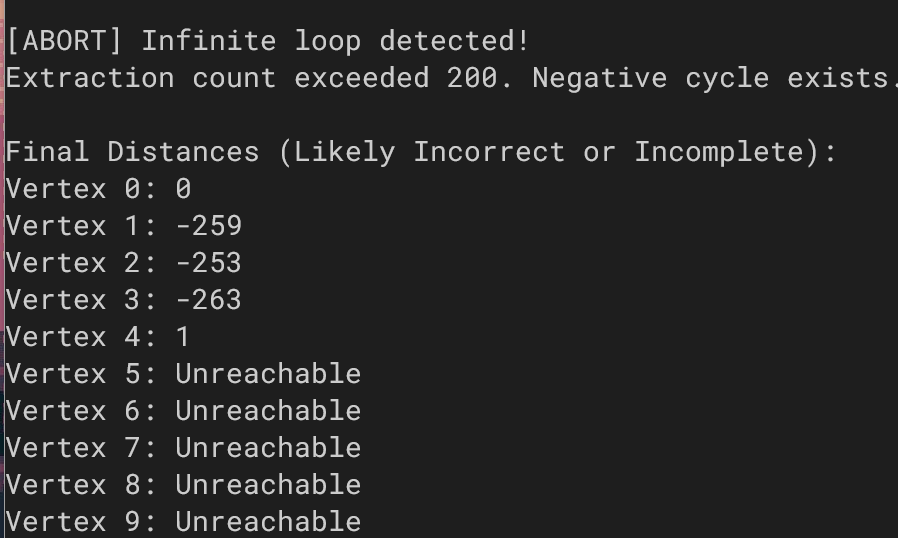
\includegraphics[width=0.9\textwidth]{Problem2/Problem2_2.png}
\end{figure}

\newpage
\subsection*{Inference}
\begin{itemize}
    \item \textbf{Algorithmic Failure:} Dijkstra's algorithm fundamentally relies on a greedy strategy, operating under the assumption that adding an edge to a path can only increase its total weight. 
    \item \textbf{Negative Edges:} When a negative edge is introduced, the algorithm may finalize a node's distance too early. A later, longer path containing a negative edge might actually result in a cheaper overall cost, which Dijkstra will ignore since the target node was already popped from the priority queue.
    \item \textbf{Negative Cycles:} In the presence of a negative weight cycle, the concept of a "shortest path" mathematically breaks down, as traversing the cycle infinitely yields an infinitely negative cost. Dijkstra has no mechanism to detect this and outputs incorrect, static values based on its initial arbitrary traversals.
\end{itemize}

\newpage

% --- Problem 3 ---
\section*{Problem 3}
\textbf{Problem Statement:} You are given a set of $n$ points: $S=\{p_{1},p_{2},...,p_{n}\}$, where $p_{i}=(x_{i},y_{i})$. Your goal is to find the pair of points $(p_{i},p_{j})$ that have the smallest distance among all pairs.

The assignment considers two cases:

\textbf{Case 1 - One-Dimensional Points (1D)} \\
Each point is represented as $p_{i}=(x_{i})$. The distance between any two points is calculated as $d=|x_{i}-x_{j}|$. You are required to find the pair of points with the minimum distance in 1D.

\textbf{Case 2 - Two-Dimensional Points (2D)} \\
Each point is represented as $p_{i}=(x_{i},y_{i})$. The distance between any two points is calculated using the Euclidean formula $d=\sqrt{(x_{i}-x_{j})^{2}+(y_{i}-y_{j})^{2}}$. You are required to find the pair of points with the minimum distance in 2D.

\textbf{Your tasks}
\begin{enumerate}
    \item Implement a method to find the closest pair of points for 1D points.
    \item Implement a method to find the closest pair of points for 2D points.
    \item Compare the time complexity of the 1D and 2D implementations.
\end{enumerate}

\newpage
\subsection*{Code}
\lstinputlisting[language=C]{Problem3/ClosestPairOfPoints1D2D.c}

\newpage
\subsection*{Output}
\begin{figure}[H]
    \centering
    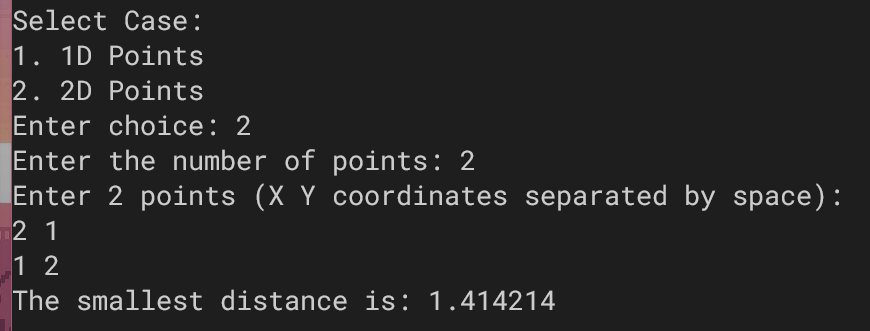
\includegraphics[width=0.9\textwidth]{Problem3/Problem 3.png}
\end{figure}

\newpage
\subsection*{Inference}
\begin{itemize}
    \item \textbf{1D Time Complexity:} The 1D approach resolves in $O(n \log n)$ time. This is achieved by sorting the array of points ($O(n \log n)$) and then performing a single linear scan ($O(n)$) to compute the distance between adjacent elements.
    \item \textbf{2D Time Complexity:} The 2D approach uses a Divide and Conquer methodology, dropping the complexity from the naive $O(n^2)$ down to $O(n \log n)$. 
    \item \textbf{Implementation Comparison:} While both algorithms share an $O(n \log n)$ time complexity bound, the 2D implementation carries a significantly larger constant factor. The 2D case requires maintaining multiple sub-arrays, recursive tree unwinding, and filtering a boundary "strip" width of $2d$ at every level of division, making it considerably heavier on memory and execution time overhead than the 1D linear scan.
\end{itemize}

\newpage

% --- Problem 4 ---
\section*{Problem 4}
\textbf{Problem Statement:} In this assignment, you are given a weighted directed graph $G=(V,E)$ where $V$ is the set of vertices and $E$ is the set of edges. Each edge $(u,v)\in E$ has a weight $w(u,v)$, which can be either positive or negative. Your task is to explore the behavior of the Bellman-Ford Algorithm when the graph contains a negative weight cycle.

The Bellman-Ford algorithm is used to find the shortest path from a source vertex $s$ to all other vertices. The distance from $s$ to any vertex $v$ is calculated as:
$$d(v)=\min_{(u,v)\in E}(d(u)+w(u,v))$$
for all edges $(u,v)\in E$.

If the graph contains a negative weight cycle (i.e., a cycle whose total weight is negative): $\sum_{(u,v)\in cycle}w(u,v)<0$, the Bellman-Ford algorithm can detect the presence of the cycle after $|V|-1$ relaxations. This is done by checking if any edge can still reduce the distance: If $d(u)+w(u,v)<d(v)$ after $|V|-1$ iterations, a negative weight cycle exists.

\textbf{Your tasks}
\begin{enumerate}
    \item Implement the Bellman-Ford algorithm for a weighted directed graph.
    \item Detect whether a negative weight cycle exists using the final relaxation check.
\end{enumerate}

\newpage
\subsection*{Code}
\lstinputlisting[language=C]{Problem4/BellmanFordAlgorithm.c}

\newpage
\subsection*{Output}
\begin{figure}[H]
    \centering
    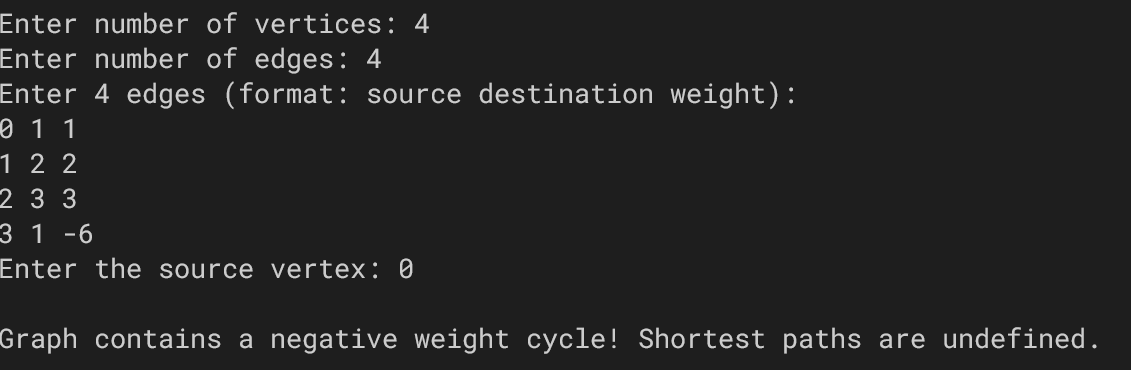
\includegraphics[width=0.9\textwidth]{Problem4/Problem 4.png}
\end{figure}

\newpage
\subsection*{Inference}
\begin{itemize}
    \item \textbf{Time Complexity:} The Bellman-Ford algorithm operates with a time complexity of $O(V \times E)$. This is because it must iterate over all $E$ edges exactly $V-1$ times to guarantee the shortest paths are found.
    \item \textbf{Handling Negative Edges:} Unlike Dijkstra's algorithm, Bellman-Ford correctly processes graphs with negative edge weights by continually relaxing edges, ensuring all potential path reductions are exhausted.
    \item \textbf{Cycle Detection:} By executing one additional ($V$-th) pass over all edges, the algorithm easily flags negative weight cycles. If the distance to any vertex is further minimized during this extra pass, it mathematically proves the existence of a negative cycle, allowing the program to safely halt and reject the undefined graph.
\end{itemize}

\newpage

% --- Appendix ---
\section*{Appendix: Header Files}
\textbf{Note:} Below are the custom header files utilized across the assignment implementations to maintain modularity.

\subsection*{MinHeap.h}
\lstinputlisting[language=C]{../Assignment_6/MinHeap/MinHeap.h}

\newpage
\subsection*{Graph.h}
\lstinputlisting[language=C]{../Assignment_6/AdjacencyList/AdjacencyList.h}

\end{document}